% Chapter Template

\chapter{Results} % Main chapter title
\textcolor{red}{add short explanations when first mentioning $\alpha$ and $q$ as reminder}

\label{chap:results} % Change X to a consecutive number; for referencing this chapter elsewhere, use \ref{ChapterX}
This chapter will summarize the results of this work. First, the results of simulating the susceptible population
in the region of Hesse will be presented. Then the results of a sensitivity analysis for the variables $\alpha$ and
$q$ will be shown. Specifically the sensitivity analysis will later be used in \hyperref[chap:discussion]{Chapter
\ref*{chap:discussion} - Discussion} to explain the results of the simulations.


%----------------------------------------------------------------------------------------
%	SECTION 1
%----------------------------------------------------------------------------------------

\section{Simulating the susceptible population of Hesse}
\label{sec:sim_res}
\textcolor{red}{check your tenses and make sure they make sense!}
\textcolor{red}{remove data point/day inconsistencies}

During this work we simulated the susceptible population of Hesse. 26 regions were simulated over a time period of
76, 60 and 50 days respectively. We will present both the absolute and percentage difference between the simulated
and the original data for each time frame.

\textcolor{red}{redo box plots with x-axis description}
\textcolor{red}{ADD OPTIMAL VALUES FOR $\alpha$ AND $q$!!}
%-----------------------------------
%	SUBSECTION 1
%-----------------------------------
\subsection{Simulating susceptibles in a 76 day time frame}
We first wanted to observe how well the simulation performs in a time frame of 76 days. Since the number of susceptible
individuals is much greater then any other group at any given data point, changes in this group can be difficult to
observe. Because of this we decided to calculate and compare the number of individuals that migrated from the susceptible
to the exposed group instead. This was done by subtracting the number of susceptible individuals at data point \I{t=x} from
the start point \I{t=0}. The result is the total change of susceptibles at any given time point, which is equivalent to the 
sum of all exposed individuals at any given time point. These results are much easier to compare and understand.
\hyperref[fig:76_sim_expl]{figure \ref*{fig:76_sim_expl}} shows three graphs that illustrate this process.


\begin{figure}
	\centering
	\begin{subfigure}[b]{0.3\textwidth}
		\centering
		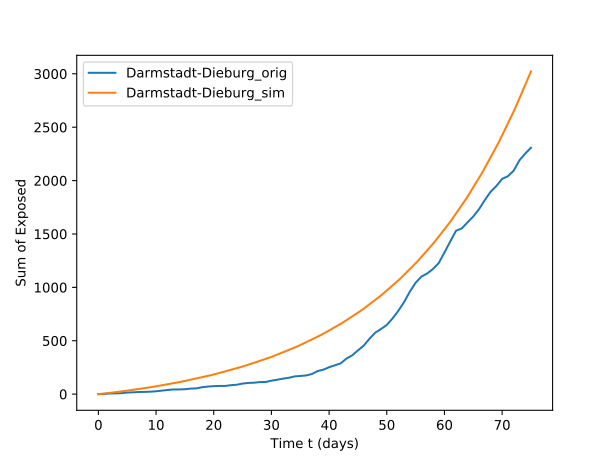
\includegraphics[width=\textwidth]{./figures/76d/24_Darmstadt-Dieburg.png}	
		\caption{}
	\end{subfigure}
	\hfill
	\begin{subfigure}[b]{0.3\textwidth}
		\centering
		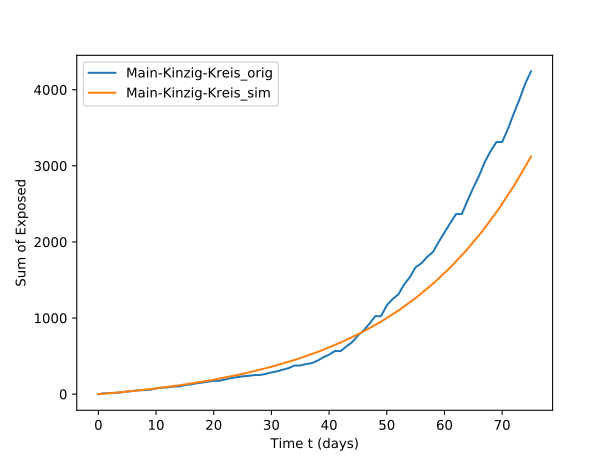
\includegraphics[width=\textwidth]{./figures/76d/13_Main-Kinzig-Kreis.png}	
		\caption{}
	\end{subfigure}
	\hfill
	\begin{subfigure}[b]{0.3\textwidth}
		\centering
		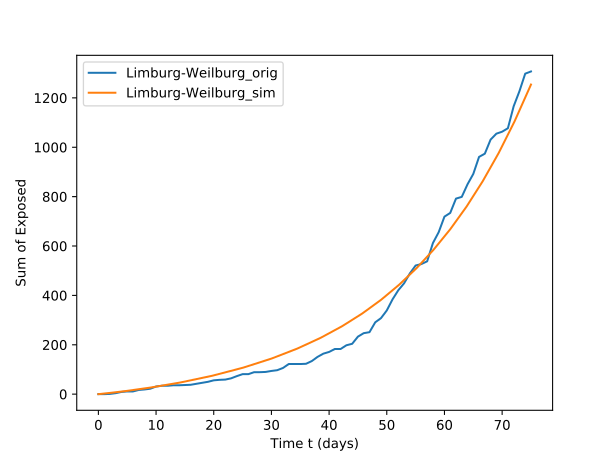
\includegraphics[width=\textwidth]{./figures/76d/10_Limburg-Weilburg.png}	
		\caption{}
	\end{subfigure}
	\caption{Three exemplary results of a simulation of the exposed individuals.
		The original (``orig'') data is drawn in blue and the simulated (``sim'') data is drawn in orange.
		The number of simulated exposed individuals can be greater (image (A), region ``Darmstadt Dieburg''), smaller 
		(image (B), region ``Mein Kinzig Kreis'') or about the same (image (C), region ``Limburg Weilburg''), as 
		the originally observed number of exposed.
		}
	\label{fig:76_sim_expl}
\end{figure}

Furthermore we analyzed the percentage deviation of original and simulated data for each time step in each region. The results
are shown in a box plot in \hyperref[fig:76_sim_box]{figure \ref*{fig:76_sim_box}}. The three regions ``Werra-Meissner-Kreis'',
``Marburg-Biedenkopf'' and ``Limburg-Weilburg'' are listed separately in figure \ref*{fig:76_sim_box}, in order to make the scales
more readable.


\begin{figure}
	\centering
	\begin{subfigure}[b]{0.4\textwidth}
		\centering
		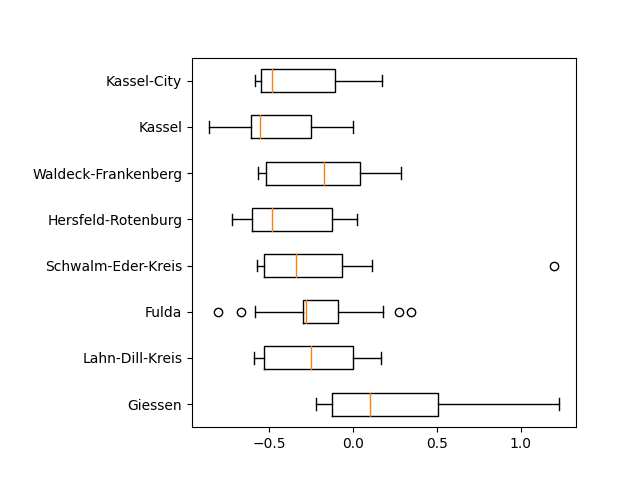
\includegraphics[width=\textwidth]{./figures/76d/deviation_box76_alt1.png}	
	\end{subfigure}
	\begin{subfigure}[b]{0.4\textwidth}
		\centering
		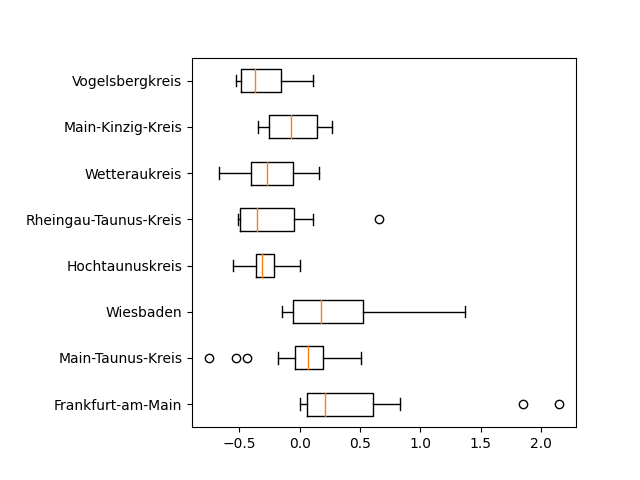
\includegraphics[width=\textwidth]{./figures/76d/deviation_box76_alt2.png}	
	\end{subfigure}
	\begin{subfigure}[b]{0.4\textwidth}
		\centering
		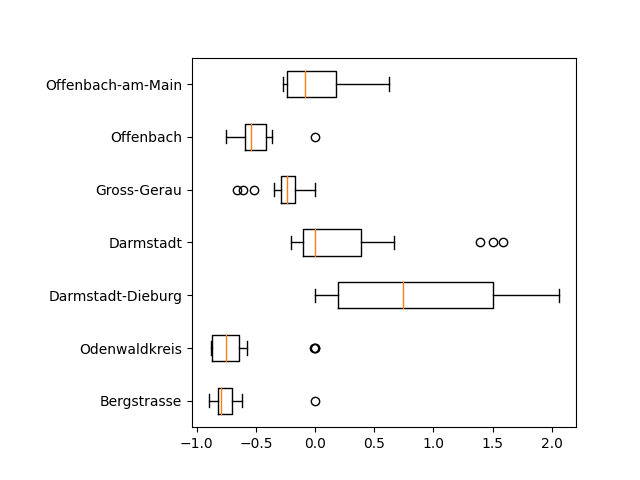
\includegraphics[width=\textwidth]{./figures/76d/deviation_box76_alt3.png}	
	\end{subfigure}
	\begin{subfigure}[b]{0.4\textwidth}
		\centering
		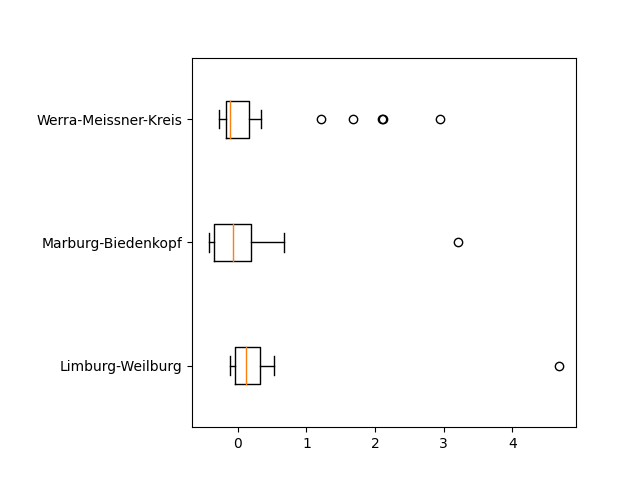
\includegraphics[width=\textwidth]{./figures/76d/deviation_box76_alt4.png}	
	\end{subfigure}
	\caption{Shown are box plots of the percentage deviation, of every simulated region relative to the original data.}
	\label{fig:76_sim_box}
\end{figure}

\textcolor{red}{rephrase for deviation factor and meaning}
Figure \ref*{fig:76_sim_box} shows that the simulated regions have a wide range of median values regarding the deviation.
The numbers are ranging between a median deviation factor of about -0.8 and +0.75. This means, that the model calculated
between 80 percent less or 75 percent more infection events, compared to the original data. 12, 21 and 25 of the 26 regions have
an absolute median deviation of less than 25, 50 and 75 percent respectively. Only the region ``Berstrasse'' had a higher deviation with
about -79.16 percent. 19 regions have a negative and 6 regions have a positive median deviation. The region ``Darmstadt'' had a
median deviation of exactly 0. Many of the plots are skewed right.
(\textcolor{red}{explain and describe better, also add data to Appendix!!!})



%-----------------------------------
%	SUBSECTION 2
%-----------------------------------
\subsection{Simulating susceptibles in a 60 day time frame}
In order to explore how well the model is working with a smaller data set, the same optimization process as in the previous section was
applied to a 60 day data set. Only the first 60 days of the previously chosen time frame were simulated, the other 16 days were
simply removed. \hyperref[fig:60_sim_expl]{Figure \ref*{fig:60_sim_expl}} shows three exemplary graphs of the simulation results.
For better comparability, the same regions were chosen as in previous section. The results were extrapolated in order to better visualize
the trend of the simulation result.

\begin{figure}
	\centering
	\begin{subfigure}[b]{0.3\textwidth}
		\centering
		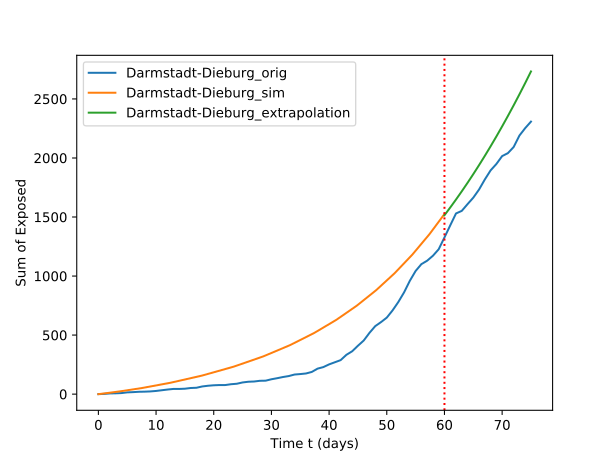
\includegraphics[width=\textwidth]{./figures/60d/24_Darmstadt-Dieburg.png}	
		\caption{}
	\end{subfigure}
	\hfill
	\begin{subfigure}[b]{0.3\textwidth}
		\centering
		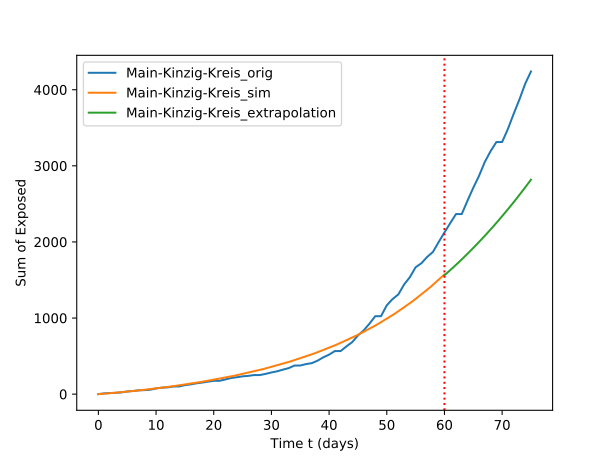
\includegraphics[width=\textwidth]{./figures/60d/13_Main-Kinzig-Kreis.png}	
		\caption{}
	\end{subfigure}
	\hfill
	\begin{subfigure}[b]{0.3\textwidth}
		\centering
		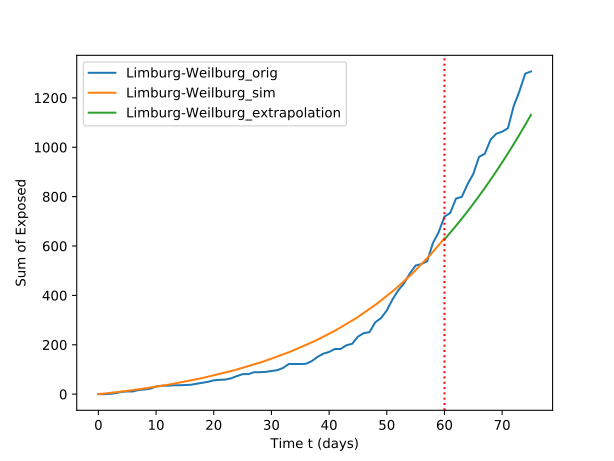
\includegraphics[width=\textwidth]{./figures/60d/10_Limburg-Weilburg.png}	
		\caption{}
	\end{subfigure}
	\caption{Three exemplary results of a simulation of the exposed individuals. The original (``orig'') data is drawn in blue,
		the simulated (``sim'') data is drawn in orange and the extrapolation of the simulated data (``extrapolation'') is
		drawn in green. The vertical red dotted line marks the transition from simulated to extrapolated data.
		}
	\label{fig:60_sim_expl}
\end{figure}

Figure \ref*{fig:60_sim_expl} shows that the general trend of the simulations remains similar to the simulations with 76 data points.
In all three regions, the extrapolated data points show a slightly slower increase in infections compared to the simulations
with 76 days in figure \ref*{fig:76_sim_expl}.

Similar to the previous section, we calculated the deviation of each data point for
each region and expressed the results in a set of box plots. The results are shown in figure \ref*{fig:60_sim_box}. Only data points
that were actually simulated were included into this analysis. Extrapolated data points were not used.

\textcolor{red}{more text for box plots}



\begin{figure}
	\centering
	\begin{subfigure}[b]{0.4\textwidth}
		\centering
		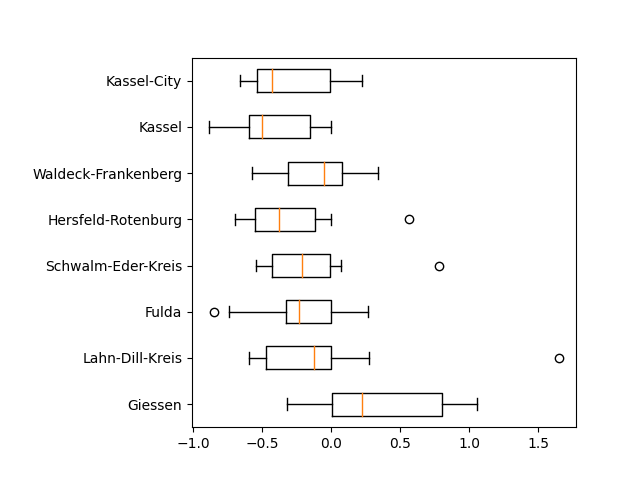
\includegraphics[width=\textwidth]{./figures/60d/deviation_box60_alt1.png}	
	\end{subfigure}
	\begin{subfigure}[b]{0.4\textwidth}
		\centering
		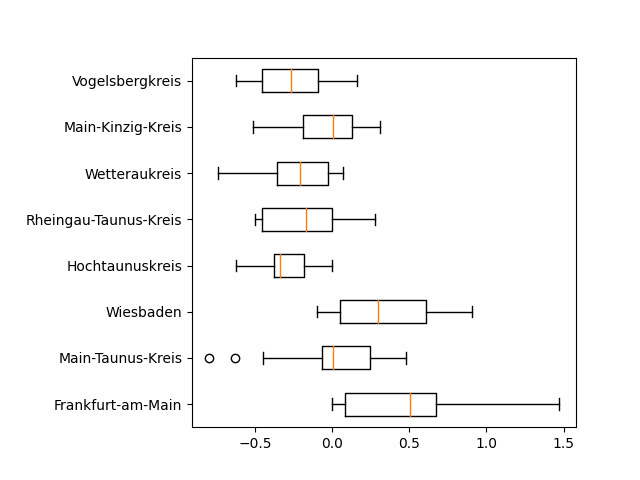
\includegraphics[width=\textwidth]{./figures/60d/deviation_box60_alt2.png}	
	\end{subfigure}
	\begin{subfigure}[b]{0.4\textwidth}
		\centering
		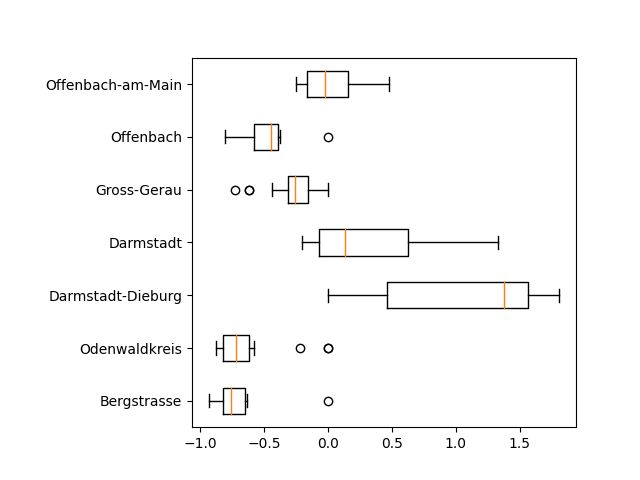
\includegraphics[width=\textwidth]{./figures/60d/deviation_box60_alt3.png}	
	\end{subfigure}
	\begin{subfigure}[b]{0.4\textwidth}
		\centering
		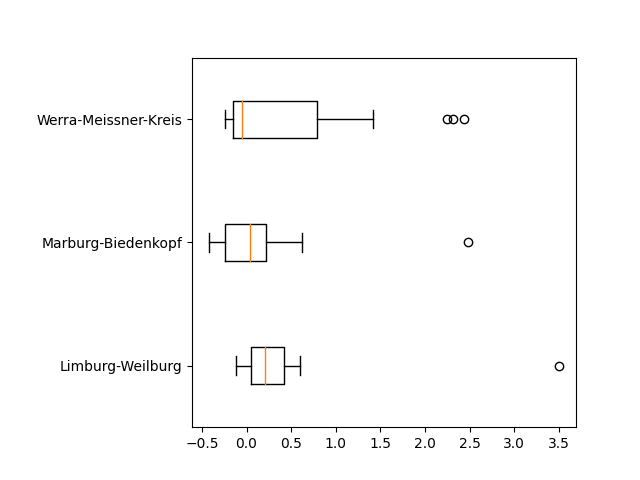
\includegraphics[width=\textwidth]{./figures/60d/deviation_box60_alt4.png}	
	\end{subfigure}
	\caption{Shown are box plots of the percentage deviation, of every simulated region relative to the original data.
		In this experiment only 60 of 76 data points were used to simulate the original data. The median of all
		simulated regions ranges between -0.76 and 1.38 and the median interquartile range is 0.41. 19 regions
		have a negative and 6 regions have a positive median deviation. The three regions ``Werra-Meissner-Kreis'',
		``Marburg-Biedenkopf'' and ``Limburg-Weilburg'' are shown separately for better scaling.
		}
	\label{fig:60_sim_box}
\end{figure}

As with the graphs described before, the deviation results of the 60 data point simulation are largely comparable to the 76
data point deviation results. The maximum and minimum median deviation of all regions is higher compared to previous results,
lying between about -76 percent and 138 percent. 14, 21 and 24 regions had an absolute, median deviation of less than
25, 50 and 75 percent respectively. The two regions with a deviation higher than 75 percent were ``Bergstrasse'' and
``Darmstadt-Dieburg'' with median deviations of -75.52 and 137.31 percent respectively.
19 of the 26 regions had a negative and 6 of the 26 regions had a positive median deviation.
As in the previous section many box plots are skewed to the right, however this effect seems to be less prominent then in
the 76 data point simulation.


%-----------------------------------
%	SUBSECTION 3
%-----------------------------------
\subsection{Simulating susceptibles in a 50 day time frame}
The last simulation that was performed, was a simulation with 50 data points. As described in the previous section with
60 data points, simulations and optimization steps were performed on a truncated data set, where the last 26 of the total
76 data points were removed. \hyperref[fig:50_sim_expl]{Figure \ref*{fig:50_sim_expl}} shows three exemplary graphs of this
experiment. As previously, the same regions were chosen as for the 76 data point experiment. 
\textcolor{red}{add more explanation and description once graphs are there}

\begin{figure}
	\centering
	\begin{subfigure}[b]{0.3\textwidth}
		\centering
		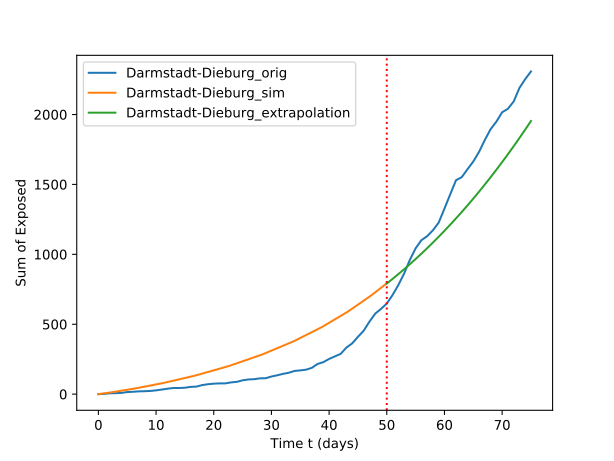
\includegraphics[width=\textwidth]{./figures/50d/24_Darmstadt-Dieburg.png}	
		\caption{}
	\end{subfigure}
	\hfill
	\begin{subfigure}[b]{0.3\textwidth}
		\centering
		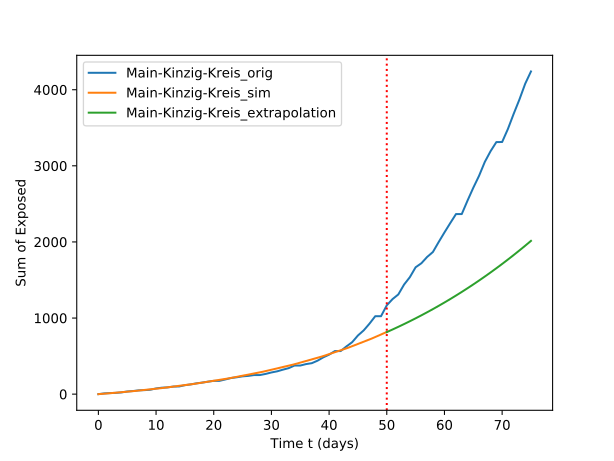
\includegraphics[width=\textwidth]{./figures/50d/13_Main-Kinzig-Kreis.png}	
		\caption{}
	\end{subfigure}
	\hfill
	\begin{subfigure}[b]{0.3\textwidth}
		\centering
		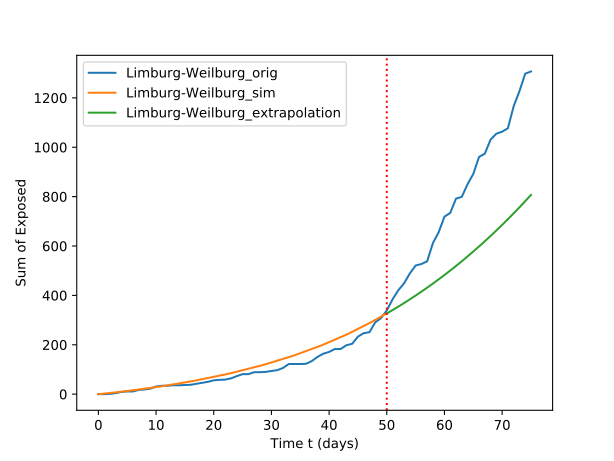
\includegraphics[width=\textwidth]{./figures/50d/10_Limburg-Weilburg.png}	
		\caption{}
	\end{subfigure}
	\caption{Add caption
		}
	\label{fig:50_sim_expl}
\end{figure}
In this experiment all three
regions show a stronger trend towards a negative deviation compared to the previous two experiments. While the regions of
the graphs, that were simulated based on the provided data points, looks similar, the overall trend visualized by
the extrapolation shows a strong deviation towards to little infections.

As with the 60 data point analysis, we also performed the deviation analysis on the 50 data point data set. As previously described
only actually simulated data points were included into the analysis. Extrapolated data points were not used. The results of this
analysis are shown in \hyperref[fig:50_sim_box]{Figure \ref*{fig:50_sim_box}}.

\begin{figure}
	\centering
	\begin{subfigure}[b]{0.4\textwidth}
		\centering
		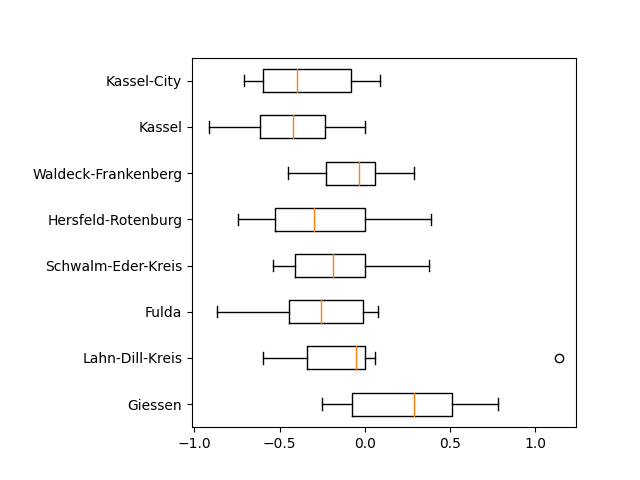
\includegraphics[width=\textwidth]{./figures/50d/deviation_box50_alt1.png}	
	\end{subfigure}
	\begin{subfigure}[b]{0.4\textwidth}
		\centering
		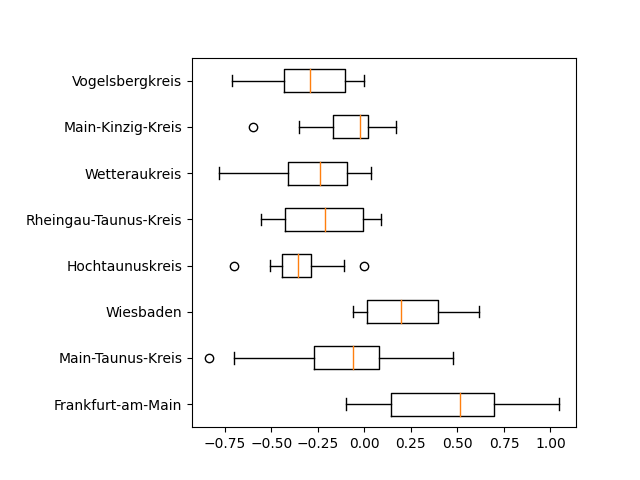
\includegraphics[width=\textwidth]{./figures/50d/deviation_box50_alt2.png}	
	\end{subfigure}
	\begin{subfigure}[b]{0.4\textwidth}
		\centering
		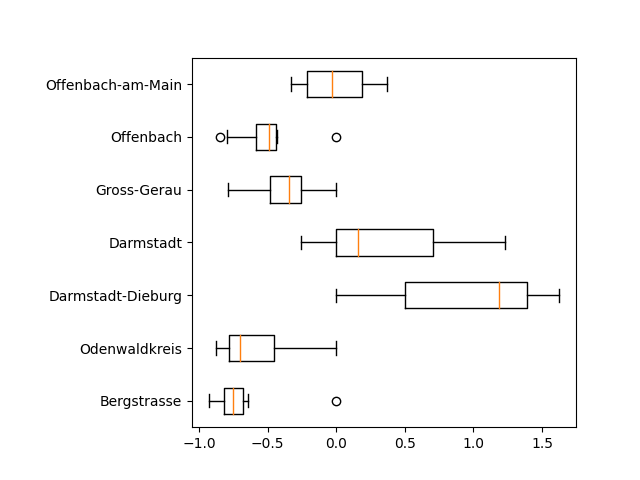
\includegraphics[width=\textwidth]{./figures/50d/deviation_box50_alt3.png}	
	\end{subfigure}
	\begin{subfigure}[b]{0.4\textwidth}
		\centering
		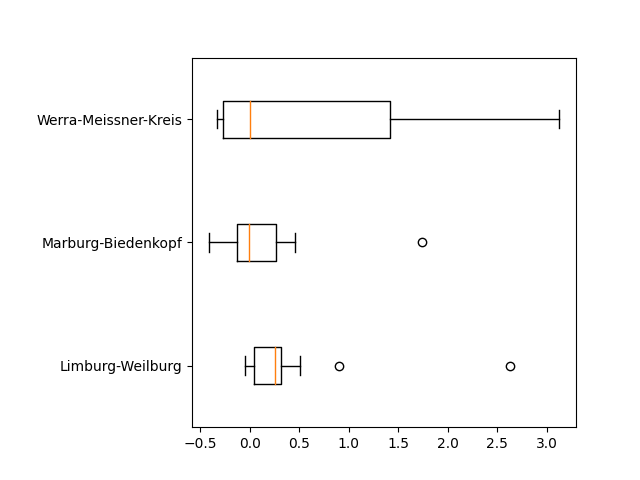
\includegraphics[width=\textwidth]{./figures/50d/deviation_box50_alt4.png}	
	\end{subfigure}
	\caption{Shown are box plots of the percentage deviation for a simulated time frame of 50 days. Each box plot includes
		all percentage deviations of all simulated data points compared to the original data. The median of all regions
		ranges between -0.76 and 1.19 and the median interquartile range is 0.38. 19 regions had a positive and
		6 regions had a negative median deviation. One region had a median deviation of exactly 0.
		The three regions ``Werra-Meissner-Kreis'', ``Marburg-Biedenkopf'' and ``Limburg-Weilburg'' are shown
		separately for better scaling.
		}
	\label{fig:50_sim_box}
\end{figure}

The 50 data point simulations show similar results to the previous two experiments. The median deviation of all regions
ranges between -76 and +119 percent and the median interquartile range is 0.38. 12, 22 and 24 regions out of 26 have an
absolute median deviation of less then 25, 50 and 75 percent respectively. The two region with a higher median
deviations are ``Bergstrasse'' and ``Darmstadt-Dieburg'', with -75.56 and 118.36 percent deviation respectively.
The skew of the box plots however is not as uniform. Many plots are skewed right like in the previous experiments, but
there is also an increased number of blots with a skew to the left. 19 of the 26 regions had a negative median deviation,
6 had a positive median deviation and one region had a median deviation of exactly 0.


%----------------------------------------------------------------------------------------
%	SECTION 2
%----------------------------------------------------------------------------------------

\section{Influence of individual regions on the loss function}
In order to better understand the influence of individual regions on the model itself, we manually calculated the total
loss, the individual loss for each region and the percentage loss of each region relative to the total loss.
\hyperref[tab:perc_region_loss]{Table \ref*{tab:perc_region_loss}} shows the results of these calculations. The table
is sorted descending from highest to lowest percentage loss contribution.
\textcolor{red}{add table with total information to Appendix}

\begin{table}
	\caption{the caption}
	\begin{tabular}{|l|x{2cm}|x{2cm}|x{2cm}|}
	%\begin{tabular}{|l|c|c|c|}
		\hline
		\B{region} & \B{percentage loss} & \B{percentage population} & \B{median deviation} \\ \hline \hline
		Offenbach & 27.70 & 5.67 & -0.54 \\ \hline
		Bergstrasse & 14.41 & 4.31 & -0.79 \\ \hline
		Frankfurt-am-Main & 13.10 & 12.14 & 0.21 \\ \hline
		Lahn-Dill-Kreis & 6.29 & 4.03 & -0.25 \\ \hline
		Main-Kinzig-Kreis & 5.17 & 6.70 & -0.07 \\ \hline
		Marburg-Biedenkopf & 4.70 & 3.91 & -0.06 \\ \hline
		Kassel-City & 3.90 & 3.19 & -0.49 \\ \hline
		Wetteraukreis & 3.35 & 4.93 & -0.27 \\ \hline
		Gross-Gerau & 2.90 & 4.38 & -0.23 \\ \hline
		Rheingau-Taunus-Kreis & 2.89 & 2.98 & -0.36 \\ \hline
		Kassel & 2.58 & 3.77 & -0.55 \\ \hline
		Hochtaunuskreis & 2.33 & 3.77 & -0.32 \\ \hline
		Darmstadt-Dieburg & 2.00 & 4.73 & 0.74 \\ \hline
		Odenwaldkreis & 1.93 & 1.54 & -0.75 \\ \hline
		Offenbach-am-Main & 1.23 & 2.08 & -0.09 \\ \hline
		Schwalm-Eder-Kreis & 1.03 & 2.86 & -0.34 \\ \hline
		Waldeck-Frankenberg & 0.99 & 2.49 & -0.17 \\ \hline
		Giessen & 0.84 & 4.32 & 0.10 \\ \hline
		Wiesbaden & 0.80 & 4.43 & 0.17 \\ \hline
		Fulda & 0.74 & 3.54 & -0.28 \\ \hline
		Hersfeld-Rotenburg & 0.41 & 1.91 & -0.48 \\ \hline
		Main-Taunus-Kreis & 0.25 & 3.80 & 0.07 \\ \hline
		Darmstadt & 0.18 & 2.53 & 0.00 \\ \hline
		Vogelsbergkreis & 0.17 & 1.68 & -0.37 \\ \hline
		Limburg-Weilburg & 0.08 & 2.74 & 0.11 \\ \hline
		Werra-Meissner-Kreis & 0.03 & 1.59 & -0.11 \\ \hline
	\end{tabular}
	\label{tab:perc_region_loss}
\end{table}

The results show, that the main contribution of the loss function is done by a minority of regions. The top three contributors
account for 55.21 percent of the entire loss, while only making up about 22.12 percent of the total population. The top seven
contributors make up about 75.27 percent, while making up about 39.95 percent of the population. A notable find is, that the
top two regions, ``Offenbach'' and ``Bergstrasse'', both display a negative deviation, while the third most influential region
``Frankfurt-am-Main'' has a positive deviation. Frankfurt also has a lower overall contribution to the loss, than the other
two regions, even though it has a higher share of the total population then the other two regions combined.

%----------------------------------------------------------------------------------------
%	SECTION 3
%----------------------------------------------------------------------------------------

\section{Sensitivity analysis of $\alpha$ and $q$}
\textcolor{red}{add more angles to the images}
In order to further investigate the features of the model, we analyzed the sensitivity of the loss function relative to
the variables $\alpha$ and $q$. We only chose those two variables, since the loss function was only calculated based
on the difference between the simulated and the original susceptible population. Since this group only depends on those
two variables in our model, changes in the other variables could not influence the loss and were therefore not investigated.
For this experiment, the 4000 simulations of the model with all 76 original data points were performed and the variables
$\alpha$ and $q$ were chosen randomly, within a set constraint. The upper and lower bounds were set to 0.05 and 0.35 for 
$\alpha$ and 5.5 and 8.0 for $q$ respectively. The results of these simulations were gathered and used to plot a map
of the variable landscape of the loss of the susceptible group.
\hyperref[fig:sensitivity_zoom0]{Figure \ref*{fig:sensitivity_zoom0}} shows the total result of all simulations over the
chosen bounds.

\begin{figure}
	\centering
	\begin{subfigure}[b]{0.4\textwidth}
		\centering
		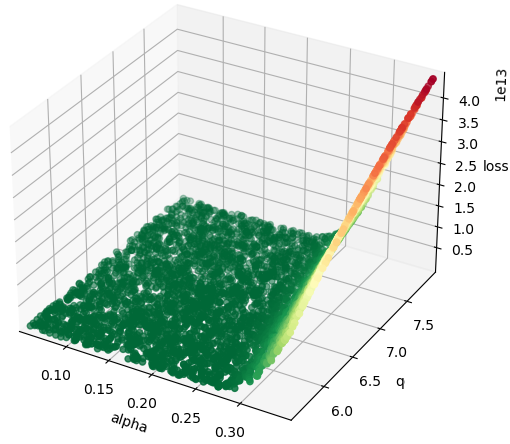
\includegraphics[width=\textwidth]{./figures/sensitivity/sensitivity_zoom0_0_2.png}	
	\end{subfigure}
	\begin{subfigure}[b]{0.4\textwidth}
		\centering
		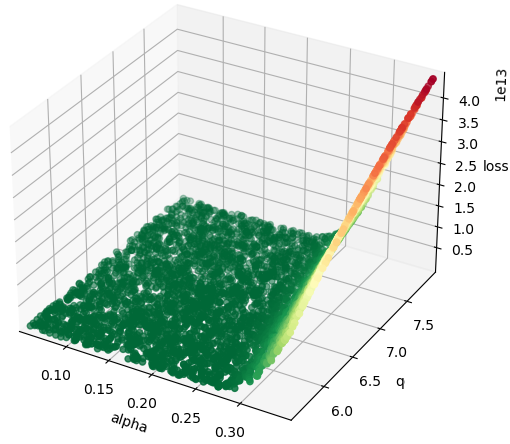
\includegraphics[width=\textwidth]{./figures/sensitivity/sensitivity_zoom0_0_2.png}	
	\end{subfigure}
	\caption{Visualization of the variable sensitivity of the susceptible group. The variables $\alpha$ and $q$ were plotted
		against the loss of the susceptible group. Images (A) and (B) show the plot from different angles in order
		to increase readability. In the model the susceptible group shows sensitivity to changes of both $\alpha$ and
		$q$. However, the sensitivity to $q$ seems to be dependent on $\alpha$.
		}
	\label{fig:sensitivity_zoom0}
\end{figure}

\textcolor{red}{add result values to figure explanation}
Figure \ref*{fig:sensitivity_zoom0} shows that low values for $\alpha$ lead to a decreased sensitivity of the loss function
for $q$. Only after an $\alpha$ value of about 0.25 is reached, does the loss start to react to changes in $q$. After this point
however, the loss function quickly increases. This phenomenon can be seen both, if $q$ is increased and if $q$ is not increased
in the simulation. But a bigger $q$ value causes the loss to increase more quickly compared to a simulation with a small loss.



The simulations were further investigated by plotting only part of the experimental data.
The first row of \hyperref[fig:sensitivity_zoom0]{Figure \ref*{fig:sensitivity_zoom0}} shows all data points with $\alpha$ values between 0.15
and 0.25, $q$ values between 5.5 and 8.0 and a maximum loss of $10^{10}$. The loss on this image was capped in order to reduce
the scale of the loss and thereby increase readability. This lead 957 of 4000 data points being plotted. The images in the
second row show the same graph (\textcolor{red}{?}), with the same bonds for $\alpha$ and $q$, but with a maximum loss capped
at $2.7*10^{9}$. This gives an even closer look at the range of optimal/close-to-optimal values for $\alpha$ and $q$.

\begin{figure}
	\centering
	\begin{subfigure}[b]{0.4\textwidth}
		\centering
		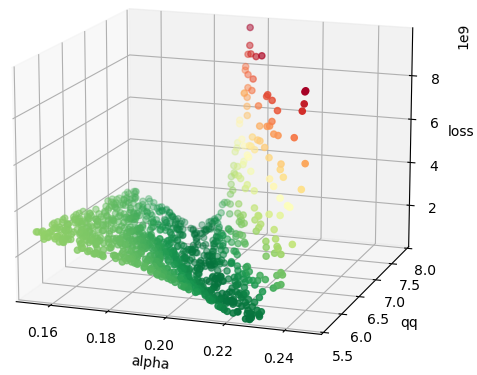
\includegraphics[width=\textwidth]{./figures/sensitivity/sensitivity_zoom1_0_2.png}	
	\end{subfigure}
	\begin{subfigure}[b]{0.4\textwidth}
		\centering
		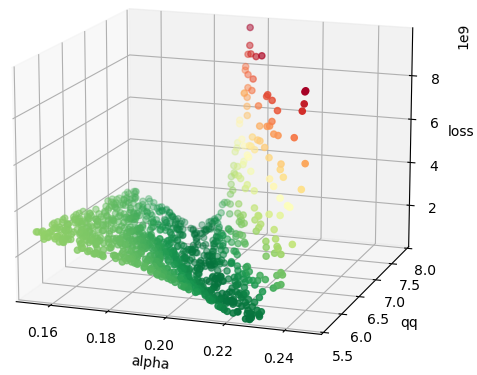
\includegraphics[width=\textwidth]{./figures/sensitivity/sensitivity_zoom1_0_2.png}	
	\end{subfigure}
	\begin{subfigure}[b]{0.4\textwidth}
		\centering
		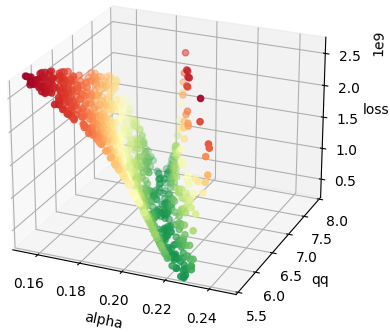
\includegraphics[width=\textwidth]{./figures/sensitivity/sensitivity_zoom2_0_2.png}	
	\end{subfigure}
	\begin{subfigure}[b]{0.4\textwidth}
		\centering
		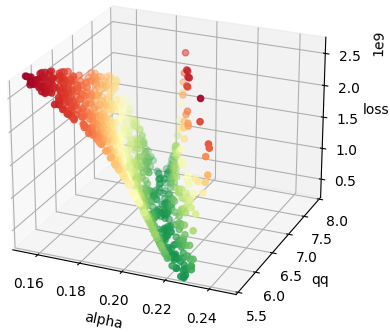
\includegraphics[width=\textwidth]{./figures/sensitivity/sensitivity_zoom2_0_2.png}	
	\end{subfigure}
	\caption{Visualization of the variable sensitivity of the susceptible group. The variables $\alpha$ and $q$ were
		capped to 0.15 and 0.25 and 5.5 and 8.0 respectively and then plotted against the result of the loss function.
		The loss was capped at $10^{10}$ and $2.7*10^{9}$ for the first and the second row respectively, in order to
		reduce the scale of the loss and make the image more readable. The image shows that there seems to be a set of
		optimal value combinations of $\alpha$ and $q$, where the loss is minimized. Given the diagonal nature of this
		``optimal cavity'' there seem to be an equilibrium between the two values.
		\textcolor{red}{check for better wording} %note
		}
	\label{fig:sensitivity_zoom1}
\end{figure}

Figure \ref*{fig:sensitivity_zoom1} shows the existence of a ``valley'' with minimized loss. It can be seen that there are 
sets of values of $\alpha$ and $q$, where the loss appears to be minimized. The optimal values found by the model for $\alpha$
and $q$ are also withing this region (\textcolor{red}{more info}). The optimized area seems to have a diagonal structure,
indicating an optimal relation between $\alpha$ and $q$.

